A continuación se presenta un análisis de la correlación entre el tiempo de ejecución de un producto matriz-matriz y los diferentes parámetros que afectan su rendimiento. El objetivo de este análisis es identificar los parámetros más relevantes en cuanto a correlación con el tiempo de ejecución y proporcionar información útil para optimizar el rendimiento del producto matriz-matriz.

Se ha calculado la matriz de correlación entre el tiempo de ejecución y los diferentes parámetros utilizando el conjunto de datos proporcionado. La matriz de correlación muestra la relación lineal entre cada par de variables. Los valores de correlación varían entre -1 y 1, donde -1 indica una correlación negativa perfecta, 0 indica ninguna correlación y 1 indica una correlación positiva perfecta. Como muestra la figura \ref{figure:corr}, los parámetros que muestran una mayor correlación con el tiempo de ejecución son MWG y NWG.

\begin{figure}[h]
    \begin{center}
        \scalebox{0.7}{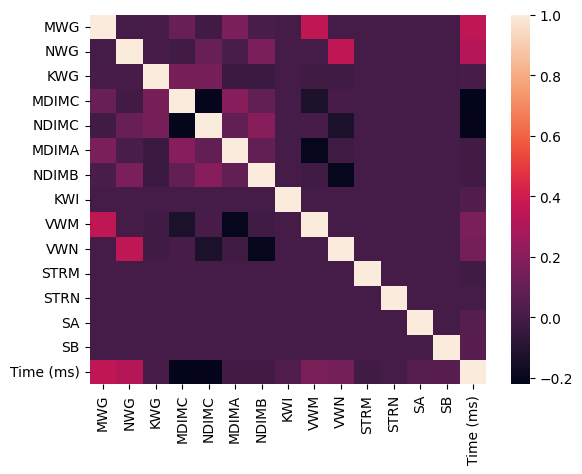
\includegraphics{corrmat.png}}
    \end{center}
    \caption{\label{figure:corr}Matriz de correlación entre todos los parámetros y el tiempo de ejecución.}
\end{figure}

También se muestra en la tabla \ref{table:corr} el índice de correlación para cada parámetro en relación con el tiempo de ejecución.

Teniendo en cuenta los valores de correlación proporcionados, se puede observar que los parámetros MWG y NWG son los más relevantes en cuanto a correlación con el tiempo de ejecución, con valores de correlación de \(0.351805\) y \(0.320455\), respectivamente. Esto indica que existe una relación positiva moderada entre estos dos parámetros y el tiempo de ejecución.

Los parámetros MDIMC y NDIMC también son relevantes en cuanto a correlación con el tiempo de ejecución, con valores de correlación de \(-0.221093\) y \(-0.214592\), respectivamente. Esto indica que existe una relación negativa moderada entre estos dos parámetros y el tiempo de ejecución.

Los demás parámetros tienen valores de correlación más bajos en valor absoluto, lo que indica que su relación con el tiempo de ejecución es más débil. En resumen, los parámetros más relevantes en cuanto a correlación con el tiempo de ejecución son MWG, NWG, MDIMC y NDIMC.

Para visualizar mejor esta relación, se han creado gráficos (figura \ref{figure:reltime}) que muestran el tiempo de ejecución en función del valor que toma cada uno de estos cuatro parámetros.

\begin{table}[h]
    \centering
    \begin{tabular}{|l|l|}
    \hline
        \textbf{Var} & \textbf{Correlation index} \\ \hline
        MWG & \textbf{0.351805} \\ 
        NWG & \textbf{0.320455} \\ 
        KWG & 0.011229 \\ 
        MDIMC & \textbf{-0.221093} \\ 
        NDIMC & \textbf{-0.214592} \\ 
        MDIMA & -0.007035 \\ 
        NDIMB & -0.008706 \\ 
        KWI & 0.032570 \\ 
        VWM & 0.164271 \\ 
        VWN & 0.144743 \\ 
        STRM & -0.012586 \\ 
        STRN & -0.000108 \\ 
        SA & 0.051974 \\ 
        SB & 0.063962 \\ 
       \textit{Time (ms)} &\textit{1.000000} \\ \hline
    \end{tabular}
    \caption{\label{table:corr}Índice de correlación entre el tiempo de ejecución y cada uno de los parámetros de entrada. Destacados los valores más relevantes.}
\end{table}

\begin{figure}[h]
    \begin{center}
        \scalebox{0.7}{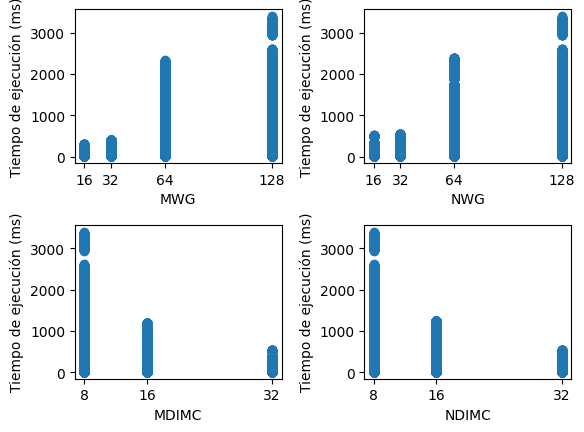
\includegraphics{paramvstime.png}}
    \end{center}
    \caption{\label{figure:reltime}Relación entre el tiempo de ejecución y los parámetros MWG, NWG, MDIMC y NDIMC.}
\end{figure}